In conclusion the practicum was really interesting to put work in. But even though the labeling performances are outstanding that solely comes from missing possibilities to test its accuracy. Also the most important drawback is the huge similarity of the training data. As written in the introduction this task asks for a method that can detect nearly any road under many different environmental conditions. There is no performance measuring done for a different environment but it is to assume that the results would be way worse. Using HOGs is a good way to get texture and color invariant information about what makes a road. But also they are not rotation-invariant what strongly limits their ability to predict in different environments. Moreover the reliance on the intensity histogram is difficult. A red brick street with a lot of shadows is a street that happens to exist often but has a entirely different intensity distribution. One possible way to improve this method would be to implement a additional on-line step which considers the last frames for the next heat map. In that you could gain speed and a sharper labeling performance.\\
\hrule
At the end we want to at least see the best classifier against one image outside the test data:
\begin{figure}[!h]
	\centering
	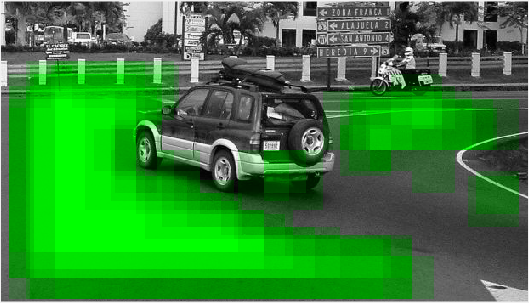
\includegraphics[width=0.4\columnwidth, keepaspectratio]{fun_pred}
	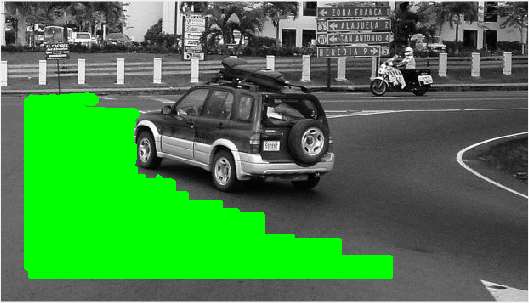
\includegraphics[width=0.4\columnwidth, keepaspectratio]{fun_morphed}
	\caption{Random toy example from the internet}
	\label{fig:fun}
\end{figure}
\hrule
\scriptsize
For computation it was always used:
\begin{itemize}
	\item[] Intel Core i5-3210M @ 2.50GHz
	\item[] 8022MB memory
	\item[] MATLAB R2015b 64-bit
\end{itemize}
